\appendix

\section{Dataset Statistics}
\label{app:dataset-stats}

\begin{figure}[t]
    \centering
    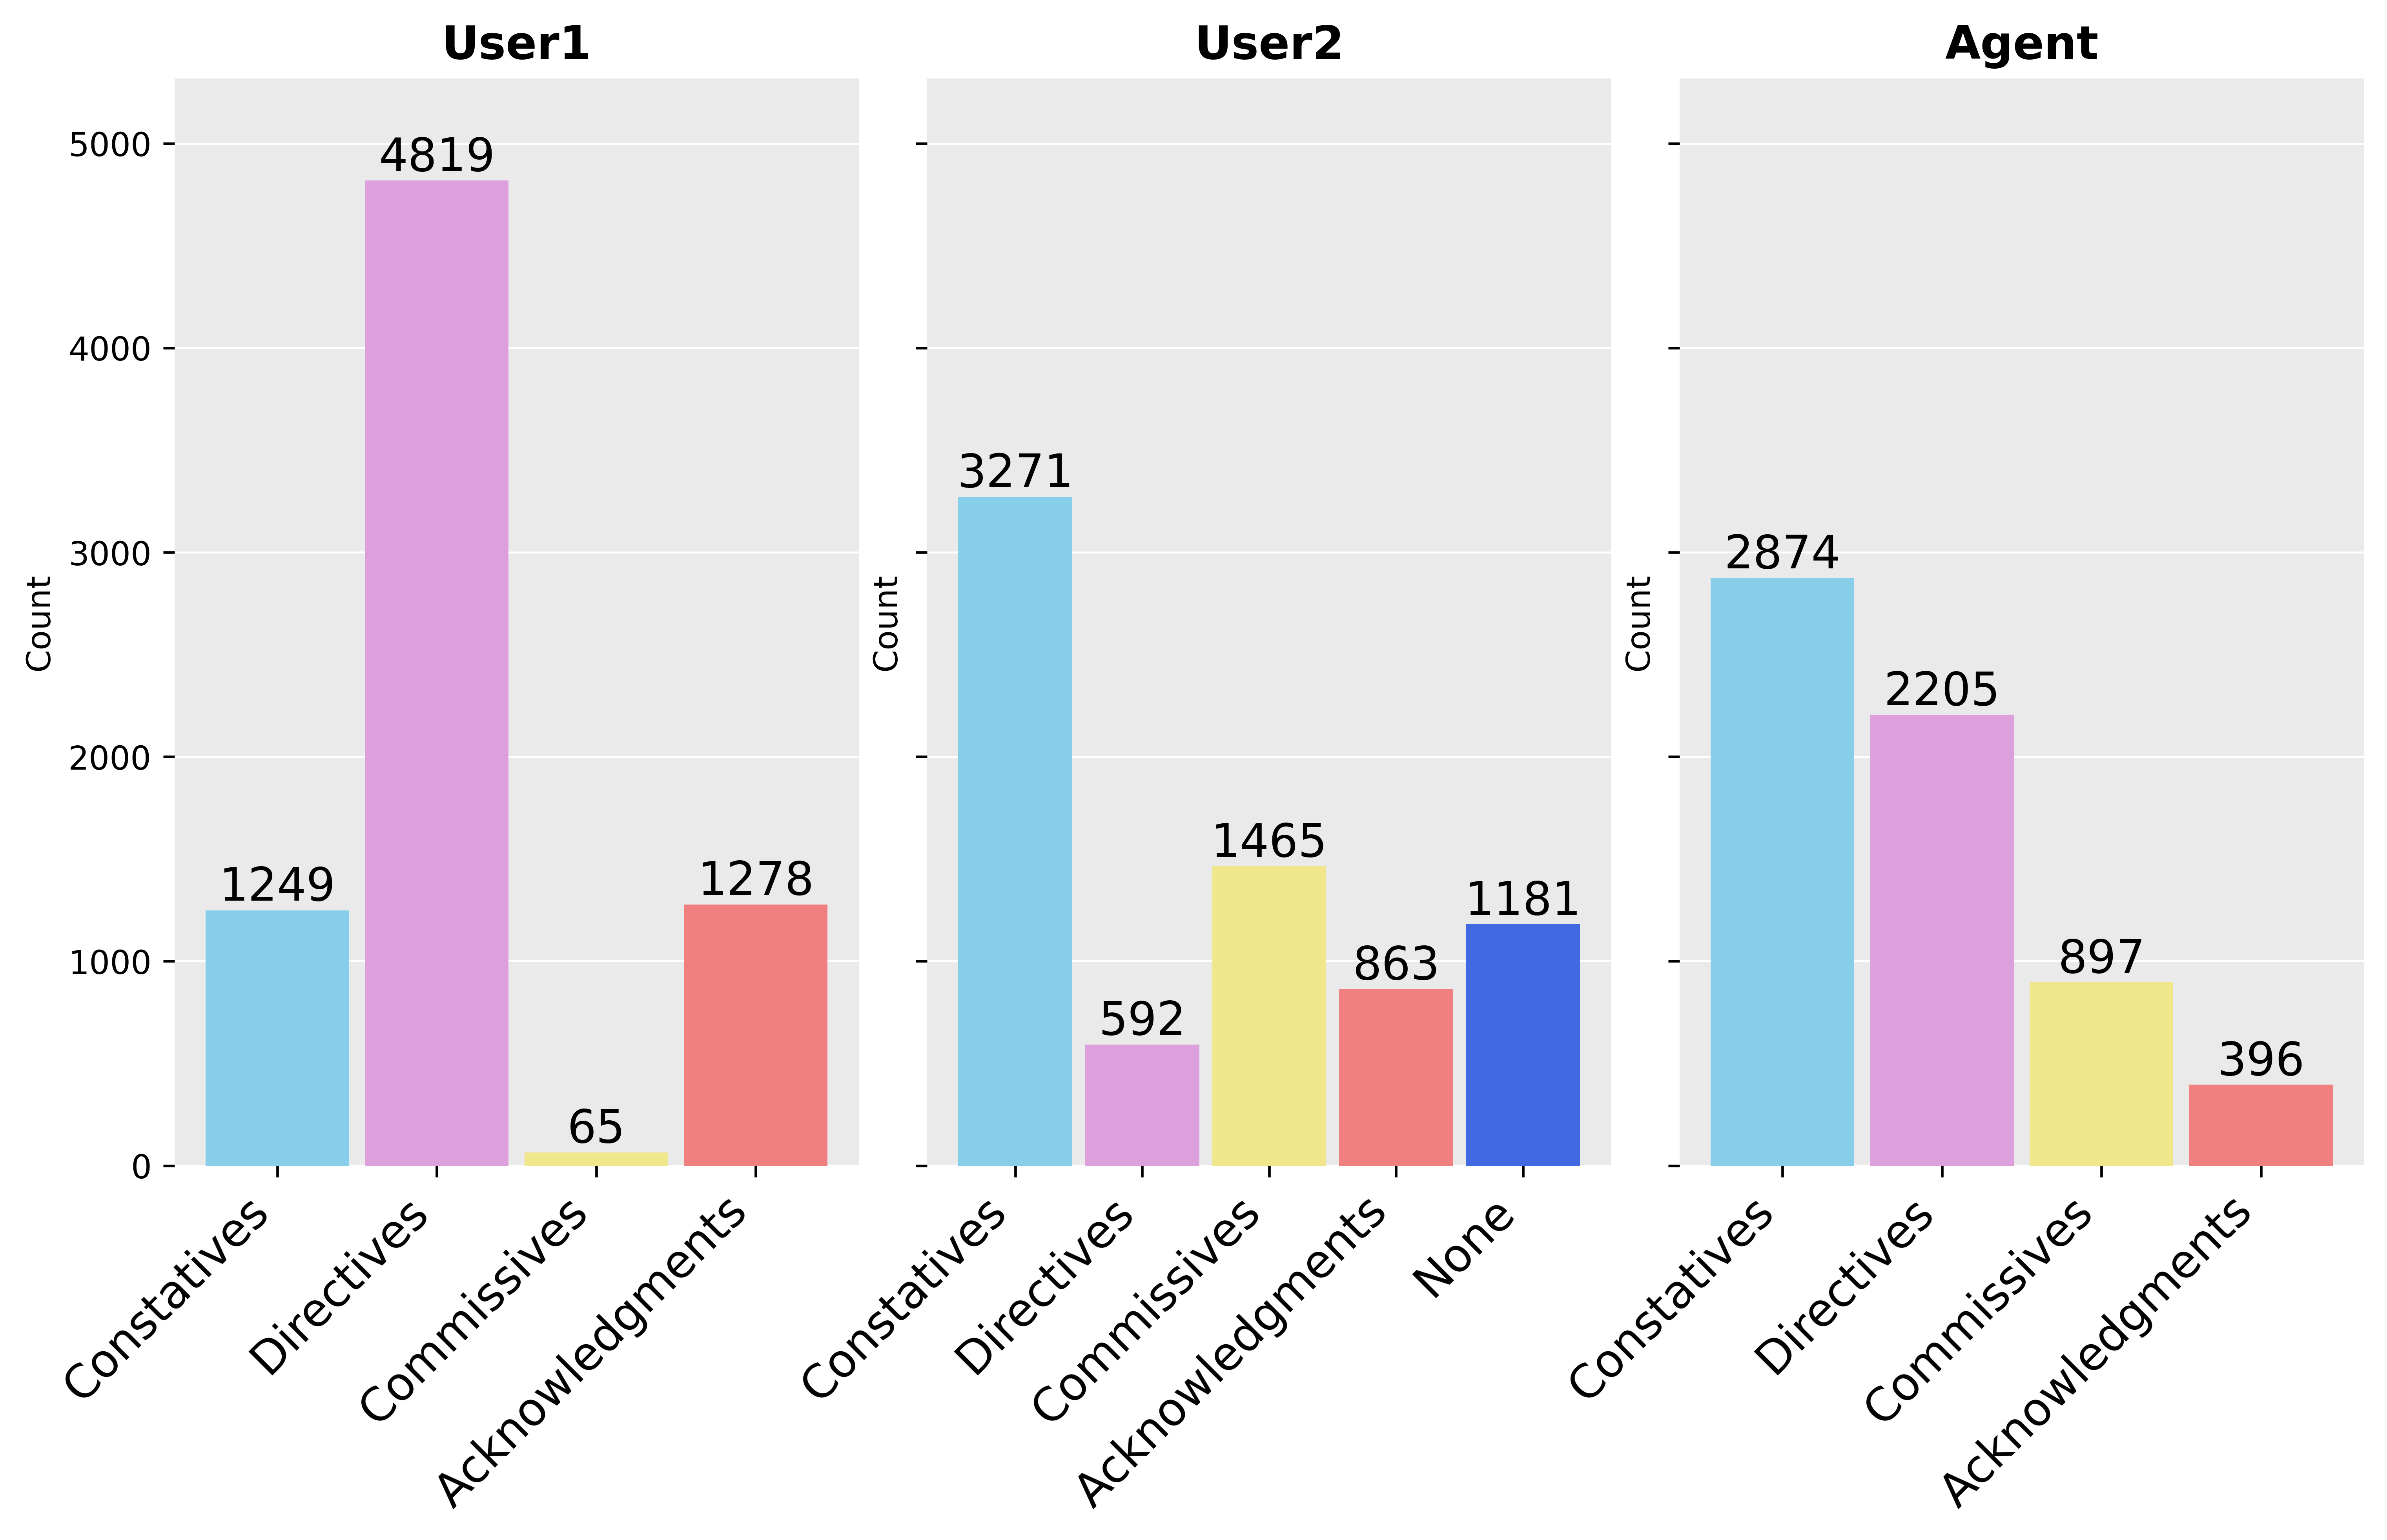
\includegraphics[width=\columnwidth]{figures/figure3.png}
    \caption{Distribution of speech acts of User$_1$, User$_2$, and Agent. We used our speech act type identification method stated in Section~\ref{sec:method-generation} to classify the speech act type of User$_1$ and Agent for comparison with User$_2$.}
\label{fig:type-distribution}
\end{figure}

% 평균적 턴의 갯수
% User2 발화의 Speech Act type의 분포 (None 포함 총 5가지, Graph로 나타낸다.)
% User2 발화의 Speech Act type별 길이 제시 - User1 발화의 평균 길이를 대상으로 해서 비교


In this section, we provide a detailed analysis of the dataset constructed for evaluating multi-user DST based on the aforementioned methodology. Our dataset is derived from the test set of MultiWOZ 2.1 \cite{eric2020multiwoz}, an existing DST benchmark. Accordingly, the dataset consists of 1,000 conversations with an average of 7.36 turns per dialogue, covering five different domains: attraction, hotel, restaurant, taxi, and train.

To examine the characteristics of multi-user interactions, we analyze the distribution of speech acts of $U^{(2)}_{t}$ within the dataset, which is depicted in Figure~\ref{fig:type-distribution}. Among all user$_2$ utterances, 44\% are constatives, 8\% are directives, 20\% are commissives, 12\% are acknowledgments, and 16\% are none (i.e., no $U^{(2)}_{t}$ at $t$).

Next, we compare the length of $U^{(2)}_{t}$ and $U^{(1)}_{t}$ in our dataset. On average, original utterances of $U^{(1)}_{t}$ contain 11.73 words, while the newly generated $U^{(2)}_{t}$ are slightly shorter, averaging 10.26 words. This difference arises because $U^{(2)}_{t}$ often consists of clarifications or brief confirmations rather than full-length requests or responses. $M_{t}$ tends to be longer, averaging 16.05 words, as they provide detailed responses or requests for clarification.

\section{Implementation Details}
\label{app:impl-details}

This section outlines implementation details to reproduce the experimental findings of our study. First, we used GPT-4o-2024-08-06 as $\mathcal{L}$ to extend the MultiWOZ 2.1 dataset, following the procedure stated in Section~\ref{sec:method-generation}. Second, for the experiment in Section~\ref{sec:experiment}, we used GPT-4o-2024-08-06, claude-3-5-sonnet-20241022, gemini-2.0-flash-001, Meta-Llama-3-8B-Instruct, and gemma-2-9b-it for each model. For hyperparameters such as temperature and top-p, we followed the default setup of each model. 

\section{Slot-Level Evaluation}
\label{app:slot-eval}

In this section, we present the experimental result measured by slot-level accuracy metrics, to supplement Section~\ref{sec:experiment-result}, which used JGA as evaluation metric \cite{dey2022towards, wang2022stop, yang2023multi, luo2024zero}. In this evaluation, we used following metrics:

\begin{itemize}
    \item \textbf{Accuracy — "None"}: Accuracy when the ground truth is "None" and the model correctly predicts "None".
    \item \textbf{Accuracy — "Dontcare"}: Accuracy when the user indicates no preference ("dontcare") and the model correctly captures it.
    \item \textbf{Accuracy — "Copy\_value"}: Accuracy when the model correctly copies a value from the user’s utterance.
    \item \textbf{Accuracy — "True"}: Accuracy when the ground truth is "true" and the model predicts "true".
    \item \textbf{Accuracy — "False"}: Accuracy when the ground truth is "false" and the model predicts "false".
    \item \textbf{Accuracy — "Refer"}: Accuracy in correctly identifying references to previously mentioned slot values.
    \item \textbf{Accuracy — "Inform"}: Accuracy in correctly predicting values explicitly provided (informed) by the user.
    \item \textbf{Slot Accuracy (SA)}: Slot Accuracy evaluates the model’s ability to correctly predict each individual (domain, slot, value) triplet at every dialogue turn. Unlike JGA, which requires the entire set of predicted belief states to exactly match the ground truth, SA compares each slot prediction independently. A prediction is counted as correct only if the domain, slot name, and slot value all match the ground truth \cite{wu2019transferable}.
\end{itemize}

The results of this analysis are presented in Table~\ref{tab:performance-slot}. They demonstrate that our findings in JGA are consistent with the slot-level metrics, which provide a more fine-grained evaluation compared to JGA. These metrics also reveal the same trend discussed in Section~\ref{sec:experiment-result}: models such as GPT-4o and Claude 3.5 Sonnet experience more pronounced performance degradation, further supporting our observations.

\begin{table*}[]
\centering
    \resizebox{\textwidth}{!}{
\begin{tabular}{l|ccccccc|cc}
\Xhline{3\arrayrulewidth}
Models                 & "None" & "Dontcare" & "Copy\_value" & "True" & "False" & "Refer" & "Inform" & SA  & JGA  \\ \hline\hline
GPT-4o                 & 94.8   & 74.6       & 90.6          & 96.6   & 89.7    & 7.8     & 64.0     & 94.4 & 57.82 \\
w/ user$_2$ utterances & -3.4   & -29.3      & -40.6         & -27.8  & -22.8   & -0.1    & -25.8    & -5.2 & -3.54 \\ \hline
Claude 3.5 Sonnet      & 96.2   & 75.9       & 93.6          & 66.8   & 87.6    & 9.7     & 63.3     & 95.7 & 62.08 \\
w/ user$_2$ utterances & -0.2   & -2.2       & -0.3          & -0.7   & -10.7   & -1.3    & -0.8     & -3.3 & -3.26 \\ \hline
Gemini-2.0-Flash       & 88.2   & 4.7        & 20.7          & 26.7   & 23.4    & 0.8     & 19.2     & 84.8 & 35.26 \\
w/ user$_2$ utterances & -0.2   & -0.2       & -0.3          & -2.7   & -0.6    & -0.3    & -0.3     & -0.2 & -2.32 \\ \hline
LLaMA-3.1-8B           & 86.0   & 27.6       & 29.1          & 39.4   & 29.0    & 5.9     & 23.4     & 83.1 & 27.96 \\
w/ user$_2$ utterances & -0.8   & -17.3      & -8.1          & -12.2  & -6.9    & -0.1    & -7.0     & -1.1 & -1.06 \\ \hline
Gemma-2-9B             & 91.3   & 34.5       & 74.8          & 60.8   & 57.2    & 15.4    & 52.8     & 90.2 & 43.52 \\
w/ user$_2$ utterances & -0.7   & -1.7       & -2.4          & -0.6   & -2.8    & -2.5    & -2.1     & -0.8 & -1.36 \\ \Xhline{3\arrayrulewidth}
\end{tabular}}
\caption{The performance of each LLM models for zero-shot DST in slot-level metrics.}
\label{tab:performance-slot}
\end{table*}

\section{Verification of Data Quality}
\label{app:verify-data-quality}
\subsection{Human Evaluation}

In this paper, we introduced a novel method for incorporating a second user’s utterance to simulate a multi-user dialogue environment. This section outlines the manual evaluation conducted to assess the quality of the generated utterances and the dataset constructed using our approach.

To perform this evaluation, we manually reviewed 100 dialogues—representing 10\% of the total dataset—based on specific criteria. Three evaluators, all volunteers from the authors’ research group, were tasked with assessing the selected dialogues according to the following dimensions:

\begin{itemize}
\item \textbf{Absence of Bias}: Identification of biased or inappropriate content in user$_2$ utterances.
\item \textbf{Utterance Quality}: Assessment of fluency and coherence within the dialogue context.
\item \textbf{Slot Consistency}: Verification that introducing user$_2$ does not inadvertently alter slot values, which would introduce noise.
\end{itemize}

The results of this evaluation are summarized in Table~\ref{tab:human-eval}. First, no instances of biased or inappropriate content were found in the reviewed dialogues, confirming that user$_2$ utterances consistently maintained a neutral and respectful tone. We attribute this to the controlled generation process, where user$_2$ responses are tightly constrained by the context provided by user$_1$.

Second, 92.68\% of user$_2$ utterances were judged as natural and contextually appropriate, indicating that our generation method effectively preserves dialogue coherence. The remaining cases exhibited minor awkward phrasing or slight tonal mismatches, but these did not significantly hinder comprehension.

Third, slot value consistency was maintained in 94.51\% of the dialogues, suggesting that the inclusion of user$_2$ rarely introduced unintended semantic shifts. In the few inconsistent cases, the discrepancies were due to subtle rephrasings that altered the slot interpretation slightly, rather than clear-cut errors. Notably, this consistency rate reflects a deliberately strict evaluation policy: evaluators were instructed to mark a slot as inconsistent whenever ambiguity was present, regardless of dataset constraints.

For example, consider the following exchange:

\begin{itemize}
\item \textbf{User1}: "I need to find a hotel that has free parking."
\item \textbf{User2}: "Make sure the hotel offers free parking for both of us."
\item \textbf{Slot}: hotel-parking = Yes
\end{itemize}

In this case, the slot was marked as inconsistent, based on the interpretation that user$_2$ implicitly requests an additional parking space. However, in MultiWOZ 2.1, the \texttt{hotel-parking} slot is binary (e.g., \texttt{yes}/\texttt{no}), and the model is not expected to distinguish between single or multiple parking requests. Thus, while human annotators may perceive this as inconsistent, such differences are typically irrelevant to the DST model. In this sense, the reported 5.49\% inconsistency rate should be viewed as an upper bound, reflecting a conservative human-centric judgment rather than an estimate of likely performance degradation (e.g., in JGA).

\begin{table}[]
\centering
    \resizebox{\columnwidth}{!}{
\begin{tabular}{l|ccc}
\Xhline{3\arrayrulewidth}
           & Absence of Bias & Utterance Quality & Slot Consistency \\ \hline
Ratio (\%) & 100.00          & 92.68             & 94.51           \\ \Xhline{3\arrayrulewidth}
\end{tabular}
}
\caption{Results of the human evaluation. A higher ratio indicates better performance.}
\label{tab:human-eval}
\end{table}

\subsection{Ablation Study on Clean Dialogues}

In addition to the human evaluation, we conducted an ablation study using 100 dialogues that had been flagged by evaluators as containing no slot inconsistencies. This experiment was carried out using GPT-4o, and the results are presented in Table~\ref{tab:performance-clean}. The findings reveal a similar pattern of performance degradation, even in these clean dialogues. This suggests that the minor inconsistencies identified during manual inspection do not significantly affect the overall conclusions of the study.



\begin{table}[]
\centering
    \resizebox{\columnwidth}{!}{
\begin{tabular}{l|ccccc|c}
\Xhline{3\arrayrulewidth}
                       & Attr. & Hotel & Rest. & Taxi & Train & Avg. \\ \hline \hline
GPT-4o                 & 39.4  & 43.4  & 60.9  & 62.8 & 62.6 & 53.82 \\
w/ user$_2$ utterances & -7.4  & -2.6  & -2.2  & -0.5 & -5.3 & -3.60 \\ \Xhline{3\arrayrulewidth}
\end{tabular}
}
\caption{Performance of GPT-4o on clean dialogues without inconsistent slots.}
\label{tab:performance-clean}
\end{table}

\section{Error Analysis}
\label{app:error-analysis}

This section provides an analysis of the errors induced by the introduction of user$_2$ utterances in multi-user DST. We manually investigated cases where the LLM correctly inferred slot values in the original dataset but misclassified them when the dataset was extended with additional user utterances. Errors primarily fall into two categories: (1) errors in extracting the correct slot value and (2) errors in identifying the correct slot type. Below, we provide examples and discussions for each type.

Table~\ref{tab:error-analysis-1} shows a conversation where the user asks for information about "Warkworth House." In the single-user scenario, the LLM correctly identifies "Warkworth House" as the value of the \textit{Hotel-Name} slot. However, once an additional user$_2$ utterance is introduced (expressing curiosity about the history of Warkworth House), the model fails to track the intended hotel name. This suggests that the extra mention of historical information deflects the model’s attention, causing it to overlook the slot value relevant to user$_1$’s primary request. Importantly, the problem seems to stem from the model’s difficulty in separating the primary user request (i.e., user$_1$ is explicitly asking for hotel details) from the ancillary utterance by user$_2$. Even though the instructions clearly state that user$_1$’s state should be tracked, the presence of another speaker’s query creates an implicit context shift. As a result, the model may conflate or ignore the critical slot values it had previously captured.

In addition to missing values, multi-user input can also cause the model to produce erroneous slot types. Table~\ref{tab:error-analysis-2} demonstrates an example where the user requests a Mediterranean restaurant. In the single-user context, the LLM assigns the \textit{Restaurant-Food} slot as "mediterranean," which is correct. However, once user$_2$ joins the conversation expressing enthusiasm for a "Mediterranean experience" in the center of town, the model additionally (and incorrectly) infers a \textit{Restaurant-Area} slot value of "dontcare." This misprediction underscores how user$_2$’s mention of a location can trigger confusion about the user’s overall constraints or preferences. The second user’s statements appear to "override" or complicate the original request, leading the model to infer a new slot type (\textit{Restaurant-Area}) even though user$_1$ never expressed indifference about the area. Such discrepancies highlight a lack of robust multi-user grounding in the model: it fails to consistently distinguish separate user$_1$ requirements from user$_2$ remarks.

These errors collectively illustrate the challenges in scaling dialogue state tracking to multi-user scenarios. Both examples suggest that LLMs struggle to track the request of primary user and disentangle the utterance of other user. In multi-user dialogue applications (e.g., group travel planning or collaborative booking platforms), these behaviors could significantly degrade user experience and system reliability. Future efforts must address how best to isolate or merge multiple users’ goals to avoid contaminating one user’s state with another’s. Potential mitigation strategies include more explicit prompts that separate user$_1$’s goals from user$_2$’s utterance, or neural architectures that model each speaker’s state in parallel and then reconcile them at the system level. Overall, our results confirm that incorporating additional speakers in dialogue amplifies existing challenges in DST, highlighting the need for further research into robust, speaker-aware state tracking mechanisms.


\begin{table}[t!]
\centering
\small

\begin{tabularx}{\columnwidth}{|X|}
\hline
\textbf{Original MultiWOZ 2.1 w/o User$_2$ Utterance}\\
\hline
\textbf{User}: Do you have information about the Warkworth House?\\
\textit{[Hotel-Name: Warkworth House]}\\

\hline
\textbf{Extended MultiWOZ 2.1 w/ User$_2$ Utterance}\\
\hline
\textbf{User1}: Do you have information about the Warkworth House?\\
\textcolor{blue}{\textbf{User2}: I'm curious about the history of Warkworth House too!}\\
\textit{[Hotel-Name: \textcolor{red}{?}]}\\

\hline

\end{tabularx}
\caption{The error case where the LLM failed to extract correct slot value when user$_2$ utterance is introduced.}
\label{tab:error-analysis-1}
\end{table}

\begin{table}[t!]
\centering
\small

\begin{tabularx}{\columnwidth}{|X|}
\hline
\textbf{Original MultiWOZ 2.1 w/o User$_2$ Utterance}\\
\hline
\textbf{Agent}: I have curry garden for Indian in the centre of town, but no south indian.\\
\textbf{User}: What about one that serves mediterranean?\\
\textit{[Restaurant-Food: mediterranean]}\\

\hline
\textbf{Extended MultiWOZ 2.1 w/ User$_2$ Utterance}\\
\hline
\textbf{Agent}: I have curry garden for Indian in the centre of town, but no south indian. \\
\textbf{User1}: What about one that serves mediterranean?\\
\textcolor{blue}{\textbf{User2}: I'm in for a Mediterranean experience. Let's explore some top-notch options in the center together!}\\
\textit{[Restaurant-Food: mediterranean, \textcolor{red}{Restaurant-Area: dontcare}]}\\

\hline

\end{tabularx}
\caption{The error case where the LLM failed to predict correct slot type when user$_2$ utterance is introduced.}
\label{tab:error-analysis-2}
\end{table}



\newpage
\onecolumn
\section{Prompt Design}
\label{app:prompt}

\subsection{Prompt for Identification of Speech Act Type}
\label{app:prompt-identification}

Note that we shuffle the order of four options for each turn, to avoid biased identification \cite{lu2022fantastically}.

\begin{figure*}[h]
    \centering
    \lstset{basicstyle=\ttfamily\tiny, breaklines=true, postbreak=\mbox{\textcolor{red}{$\hookrightarrow$}\space}}
\begin{lstlisting}
Examine the previous dialogue history and choose the appropriate strategy for the utterance of User2 among the four options below. Considering the previous conversation, choose appropriate, unbiased representation for diversity.

Dialogue history so far:
{DIALOGUE HISTORY}

Current turn:
Agent: {AGENT UTTERANCE}
User1: {USER1 UTTERANCE}
User2: <New utterance to be generated>

Your task and requirements:
- Select one option among the four options mentioned below: 
    - Constatives : committing the speaker to something's being the case (answering, claiming, confirming, denying, disagreeing, stating)
    - Directives : attempts by the speaker to get the addressee to do something (apologizing, greeting, thanking, accepting an acknowledgment)
    - Commissives : committing the speaker to some future course of action (advising, asking, forbidding, inviting, ordering, requesting)
    - Acknowledgments : express the speaker's attitude regarding the hearer with respect to social action (promising, planning, vowing, betting, opposing)
- Output must be same words in prompt type option "Constatives", "Directives", "Commissives", "Acknowledgments".

\end{lstlisting}
\end{figure*}

\subsection{Prompt for Utterance Generation}
\label{app:prompt-generation}

\begin{figure*}[h]
    \centering
    \lstset{basicstyle=\ttfamily\tiny, breaklines=true, postbreak=\mbox{\textcolor{red}{$\hookrightarrow$}\space}}
\begin{lstlisting}
You are User2, a friend of User1. Your role is to casually communicate with User1 between Agent in less than 20 words following generation guide. User1 and User2 are talking to Agent.

Dialogue history so far:
{DIALOGUE HISTORY}

Current turn:
User1: {USER1 UTTERANCE}
User2: <New utterance to be generated>
Fixed slots: {SLOT VALUE OF CURRENT TURN}

Your task and requirements:

- Generate an appropriate utterance for User2 to respond to User1.
- Do not modify existing Current fixed slot and values or introduce new slot and values.
- Do not generate repeated utterances. (Ex. starting with 'Let's'or 'That sounds')
- Do not ask questions to User1. Only ask to Agent. Because the Agent will respond in the next turn.\n"
- Do not mention explitcitly word 'Agent'.\n"
- Note that you are in same circumstances with User1.
- Types of generated dialogues of User2: {UTTERANCE TYPE}

\end{lstlisting}
\end{figure*}

\subsection{Prompt for Validation of Generated Utterance}
\label{app:prompt-validation}

\begin{figure*}[h]
    \centering
    \lstset{basicstyle=\ttfamily\tiny, breaklines=true, postbreak=\mbox{\textcolor{red}{$\hookrightarrow$}\space}}
\begin{lstlisting}

You will be given a conversation sequence consisting of three parts:
1. Agent's response to previous Generated_User1 (`A`): {AGENT UTTERANCE}
2. User1's original utterance (`U1`): {USER1 UTTERANCE}
3. Generated_User2's transformed utterance (`U2`): {USER2 UTTERANCE}

Your task is to check the consistency of the sequence:
1. Check if User2's utterance (`U2`) is logically consistent with User1's original utterance (`U1`).
2. Verify that Generated_User2's (`U2`) slots match the current slot values from User1 (`U1`) slot: {SLOT VALUE OF CURRENT TURN}.
Output 'True' if both criteria 1 and 2 are met. Otherwise, output 'False'. Output: [True / False]

\end{lstlisting}
\end{figure*}

\newpage
\subsection{Prompt for Experiment}
\label{app:prompt-experiment}

Note that this is a slightly updated version of the prompt design suggested by previous study, considering the existence of user$_2$ \cite{heck2023chatgpt}.

\begin{figure*}[h]
    \centering
    \lstset{basicstyle=\ttfamily\tiny, breaklines=true, postbreak=\mbox{\textcolor{red}{$\hookrightarrow$}\space}}
\begin{lstlisting}
Consider the following list of concepts, called "slots" provided to you as a json list.

"slots": {   
    "taxi-leaveAt": "the departure time of the taxi",
    "taxi-destination": "the destination of the taxi",
    "taxi-departure": "the departure of the taxi",
    "taxi-arriveBy": "the arrival time of the taxi",
    "restaurant-book_people": "the amount of people to book the restaurant for",
    "restaurant-book_day": "the day for which to book the restaurant",
    "restaurant-book_time": "the time for which to book the restaurant",
    "restaurant-food": "the food type of the restaurant",
    "restaurant-pricerange": "the price range of the restaurant",
    "restaurant-name": "the name of the restaurant",
    "restaurant-area": "the location of the restaurant",
    "hotel-book_people": "the amount of people to book the hotel for",
    "hotel-book_day": "the day for which to book the hotel",
    "hotel-book_stay": "the amount of nights to book the hotel for",
    "hotel-name": "the name of the hotel",
    "hotel-area": "the location of the hotel",
    "hotel-parking": "does the hotel have parking",
    "hotel-pricerange": "the price range of the hotel",
    "hotel-stars": "the star rating of the hotel",
    "hotel-internet": "does the hotel have internet",
    "hotel-type": "the type of the hotel",
    "attraction-type": "the type of the attraction",
    "attraction-name": "the name of the attraction",
    "attraction-area": "the area of the attraction",
    "train-book_people": "the amount of people to book the train for",
    "train-leaveAt": "the departure time of the train",
    "train-destination": "the destination of the train",
    "train-day": "the day for which to book the train",
    "train-arriveBy": "the arrival time of the train",
    "train-departure": "the departure of the train"
}

Some "slots" can only take a value from predefined list:

"categorical": {
    "hotel-pricerange": ["cheap", "moderate", "expensive"],
    "hotel-area": ["north", "south", "east", "west", "centre"],
    "hotel-parking": ["yes", "no"],
    "hotel-internet": ["yes", "no"],
    "hotel-type": ["hotel", "guest house"],
    "restaurant-pricerange": ["cheap", "moderate", "expensive"],
    "restaurant-area": ["north", "south", "east", "west", "centre"],
    "attraction-area": ["north", "south", "east", "west", "centre"]
}

Now consider the following dialogue between more than two parties called the "system", "user1", and "user2".

Can you make answer as JSON ouput format which of the "slots" were updated by the "user1" in its latest response to the "system" refer to "slots" JSON list?

Present the updates in JSON format for each "slot" that was updated. There has no more than one update per "slot".
If no "slots" were updated, return an empty JSON list. If you encounter "slots" that were requested by the "user1" then fill them with "?". If a user does not seem to care about a discussed "slot" fill it with "dontcare".

\end{lstlisting}
\end{figure*}

% 아래첨자에 t시점마다를 빼었음. U_t 와 혼용되지 않도록 윗첨자에 화자순서를 표기
% \begin{algorithm}
% \caption{User$_2$ Utterance Generation}
% \begin{algorithmic}[1]
% \Require Chat history $H$, User$_1$ utterance $U^1$, Agent response $A$, Slot info $S$, Retries $k$
% \Ensure Generated User$_2$ utterance $U^2$ or $\emptyset$

% \State Initialize $H$
% \State Determine speech act type $D$ from $A$, $U^1$
% \State Construct prompt $P$ using $H$, $A$, $U^1$, $D$, $S$
% \For{$i = 1$ to $k$}
%     \State Generate $U^2$ using $P$
%     \If {$U^2$ is valid}
%         \State \Return $U^2$ 
%     \EndIf
% \EndFor
% \State \Return $\emptyset$
% \end{algorithmic}
% \end{algorithm}


% \begin{gather*}
% A_1 = P \oplus \text{``agent'': } M_1 \oplus \text{``user1'': } U_1^1 
% \oplus \text{``user2'': } U_1^2 \text{ if } U_1^2 \neq \emptyset,\\ 
% A_t = \text{``agent'': } M_t \oplus \text{``user1'': } U_1^1 
% \oplus \text{``user2'': } U_1^2 \text{ if } U_1^2 \neq \emptyset,\\ 
% \forall t \in [2, T].
% \end{gather*}